%-------------------------------------------------------------------------------
\section{Signal and background modelling}
\label{sec:signal_background_model}
%-------------------------------------------------------------------------------

Signal and most background processes are modelled using Monte Carlo (MC) simulation.
After the event preselection, the main background is $\ttbar$ production, often in association with jets, denoted by $\ttbar$+jets in the following.
Small contributions arise from single-top-quark, $W/Z$+jets, multijet and diboson ($WW,WZ,ZZ$) production, as well as from the associated 
production of a vector boson $V$ ($V=W,Z$) or a Higgs boson and a $\ttbar$ pair ($\ttbar V$ and $\ttbar H$). All backgrounds 
with prompt leptons, i.e. those originating from the decay of a $W$ boson, a $Z$ boson, or a $\tau$-lepton,
are estimated using samples of simulated events and initially normalised to their theoretical cross sections.
In the simulation, the top-quark and SM Higgs boson masses are set to $172.5~\gev$ and $125~\gev$, respectively,
and the Higgs boson is allowed to decay into all SM particles with branching ratios calculated using \textsc{Hdecay}~\cite{Djouadi:1997yw}.  
Backgrounds with non-prompt electrons or muons, with photons or jets misidentified as electrons, or with jets misidentified as $\had$ candidates, 
generically referred to as fake leptons, are estimated using data-driven methods. 
The background prediction is further improved during the statistical analysis by performing a likelihood 
fit to data using several signal-depleted analysis regions, as discussed in Sections~\ref{sec:strategy_Hbb} and~\ref{sec:strategy_Htautau}.

%-------------------------------------------------------------------------------
\subsection{Simulated signal and background processes}
\label{sec:simulations}
%-------------------------------------------------------------------------------

Samples of simulated $\ttbar \to WbHq$ events were generated with the next-to-leading-order (NLO) generator\footnote{In the following, 
the order of a generator should be understood as referring to the order in the strong coupling constant at which the matrix-element calculation 
is performed.} {\amcatnlolong}~2.4.3~\cite{Alwall:2014hca}  (referred to in the following as {\amcatnlo}) with the NNPDF3.0 NLO~\cite{Ball:2014uwa} parton distribution function (PDF) set and interfaced to {\pythia} 8.212~\cite{Sjostrand:2007gs} with the NNPDF2.3 LO~\cite{Ball:2012cx} PDF set for the modelling of parton showering, hadronisation, and the underlying event. 
The A14~\cite{ATLASUETune4} set of tuned parameters in {\pythia} controlling the description of multiparton interactions and  
initial- and final-state radiation, referred to as the tune, was used.
The signal sample is normalised to the same total cross section as used for the inclusive $t\bar{t}\to WbWb$ sample (see discussion below) and
assuming an arbitrary branching ratio of $\BR_{\mathrm{ref}}(t\to Hq)=1\%$.
The case of both top quarks decaying into $Hq$ is neglected in the analysis given the existing upper limits on $\BR(t \to Hq)$ (Section~\ref{sec:intro}).

The nominal sample used to model the $\ttbar$ background was generated with the NLO generator {\powheg}~v2 \cite{Frixione:2007nw,Nason:2004rx,Frixione:2007vw,Alioli:2010xd} using the NNPDF3.0 NLO PDF set. The {\powheg} model parameter $h_{\textrm{damp}}$, which controls 
matrix element to parton shower matching and effectively regulates the high-$\pt$ radiation, was set to 1.5 times the top-quark mass. 
Parton shower, hadronisation, and underlying event were modelled by {\pythia}~8.210 with the NNPDF2.3 LO PDF set in combination with the A14 tune.
Alternative $\ttbar$ simulation samples used to derive systematic uncertainties are described in Section~\ref{sec:syst_bkgmodeling}. 
The generated $\ttbar$ samples are normalised to a theoretical cross section of $832^{+46}_{-51}$~pb, 
computed using \textsc{Top++}~v2.0~\cite{Czakon:2011xx} at next-to-next-to-leading order (NNLO), 
including resummation of next-to-next-to-leading logarithmic (NNLL) soft gluon 
terms~\cite{Cacciari:2011hy,Baernreuther:2012ws,Czakon:2012zr,Czakon:2012pz,Czakon:2013goa}.
%and using the MSTW 2008 NNLO~\cite{Martin:2009iq,Martin:2009bu} PDF set. 
%The theoretical uncertainties result from variations of the factorisation and renormalisation scales, as well as from uncertainties in the
%top quark mass, and in the PDF and $\alpha_{\textrm{S}}$. The latter two represent the largest contribution to the overall theoretical uncertainty 
%in the cross section and were calculated using the PDF4LHC prescription~\cite{Botje:2011sn} 
%with the MSTW 2008 68\% CL NNLO, CT10 NNLO~\cite{Lai:2010vv,Gao:2013xoa} and NNPDF2.3 5F FFN~\cite{Ball:2012cx} PDF sets.

%The $\Hbb$ search requires a more sophisticated treatment of the $\ttbar$ background. 
The $\ttbar$ background selected by the $\Hbb$ search is enriched in $\ttbar$+heavy-flavour production, and thus requires a more sophisticated 
treatment than provided by the nominal $\ttbar$ sample, which is briefly outlined below. A detailed discussion can be found in Ref.~\cite{Aaboud:2017rss}.
%The large and complex $\ttbar$ background selected by the $\Hbb$ search requires a more sophisticated treatment than provided by the nominal $\ttbar$ sample. 
The simulated $\ttbar$ events are categorised depending 
on the flavour content of additional particle jets not originating from the decay of the $\ttbar$ system.
Events labelled as either \ttbin\ or \ttcin\ are generically referred to in the following as $\ttbar$+HF events, where HF stands for heavy flavour.
The remaining events are labelled as $\ttbar$+light-jets events, including those with no additional jets. 
A finer categorisation of \ttbin\ events is considered for the purpose of applying further corrections and
assigning systematic uncertainties associated with the modelling of heavy-flavour production in different event topologies~\cite{Aaboud:2017rss}.
In particular, the \ttbin\ events are reweighted to an NLO prediction in the four-flavour (4F) scheme 
of \ttbin\ production including parton showering~\cite{Cascioli:2013era}, based on {\ShOLlong}~\cite{Gleisberg:2008ta, Cascioli:2011va} (referred to as {\ShOL} 
in the following) using the CT10 4F PDF set.  This reweighting is performed in such a way that the inter-normalisations of the \ttbin\ categories are at NLO accuracy, 
while preserving the \ttbin\ cross section of the nominal $\ttbar$ sample. 
%This reweighting is applied to the alternative $\ttbar$ samples as well.
This reweighting is also applied to the alternative $\ttbar$ samples that are used to study systematic uncertainties.

Samples of single-top-quark events corresponding to the $t$-channel production mechanism were generated with the 
{\powheg}~v1~\cite{Frederix:2012dh} generator that uses the 4F scheme  for the NLO matrix-element calculations
and the fixed 4F \textsc{CT10}f\textsc{4}~\cite{Lai:2010vv} PDF set.
Samples corresponding to the $tW$- and $s$-channel production mechanisms were generated 
with {\powheg}~v1 using the CT10 PDF set. Overlaps between the $\ttbar$ and $tW$ final states were avoided by using 
the diagram removal scheme~\cite{Frixione:2005vw}.
The parton shower, hadronisation and the underlying event were modelled using {\pythia}~6.428~\cite{Sjostrand:2006za} 
with the CTEQ6L1~\cite{Pumplin:2002vw,Nadolsky:2008zw} PDF set 
in combination with the Perugia 2012 tune~\cite{Skands:2010ak}.
The single-top-quark samples are normalised to the approximate NNLO theoretical cross 
sections~\cite{Kidonakis:2011wy,Kidonakis:2010ux,Kidonakis:2010tc}. 

Samples of $W/Z$+jets events were generated with the {\sherpa}~2.2.1~\cite{Gleisberg:2008ta} generator. 
The matrix element was calculated for up to two partons at NLO and up to four partons at LO using 
\textsc{Comix}~\cite{Gleisberg:2008fv} and \textsc{OpenLoops}~\cite{Cascioli:2011va}. The matrix-element calculation 
is merged with the {\sherpa} parton shower~\cite{Schumann:2007mg} using the ME+PS@NLO prescription~\cite{Hoeche:2012yf}. 
The PDF set used for the matrix-element calculation is NNPDF3.0 NNLO~\cite{Ball:2014uwa} with a dedicated parton shower tuning developed for {\sherpa}. 
Separate samples were generated for different $W/Z$+jets categories using filters for a $b$-jet 
($W/Z$+$\geq$1$b$+jets), a $c$-jet and no $b$-jet ($W/Z$+$\geq$1$c$+jets), and with a veto on $b$- and $c$-jets 
($W/Z$+light-jets), which are combined into the inclusive $W/Z$+jets samples.
Both the $W$+jets and $Z$+jets samples are normalised to their respective inclusive NNLO theoretical 
cross sections calculated with \textsc{FEWZ}~\cite{Anastasiou:2003ds}.

Samples of $WW/WZ/ZZ$+jets events were generated with {\sherpa}~2.2.1 using the CT10 PDF set
and include processes containing up to four electroweak vertices. 
In the case of $WW/WZ$+jets ($ZZ$+jets) the matrix element was calculated for zero (up to one) additional partons 
at NLO and up to three partons at LO using the same procedure as for the $W/Z$+jets samples. 
The final states simulated require one of the bosons to decay leptonically and the other hadronically.
All diboson samples are normalised to their NLO theoretical cross sections provided by {\sherpa}. 

Samples of $\ttbar V$ and $\ttbar H$ events were generated with {\amcatnlo}~2.2.1, using NLO matrix elements and the NNPDF3.0 NLO PDF set,
and interfaced to {\pythia}~8.210 with the NNPDF2.3 LO PDF set and the A14 tune. 
Instead, the $\ttbar V$ samples used in the $\Hbb$ search are based on LO matrix elements computed for up to two additional partons 
using the NNPDF3.0 NLO PDF set, and merged using the CKKW-L approach~\cite{Lonnblad:2001iq}.
The $\ttbar V$ samples are normalised to the NLO cross section computed with {\amcatnlo}, while the $\ttbar H$ sample is normalised using 
the NLO cross section recommended in Ref.~\cite{deFlorian:2016spz}.
%Raitio:1978pt,Beenakker:2002nc,Dawson:2003zu,Yu:2014cka,Frixione:2015zaa}. 

%The production of four-top-quark events in the SM was simulated by samples generated at LO using {\amcatnlo}~2.2.2
%and the NNPDF2.3 LO PDF set, interfaced to {\pythia}~8.186 in combination with the A14 tune. 
%The sample was normalised to a cross section of 9.2 fb, computed at NLO~\cite{Alwall:2014hca}.

All generated samples, except those produced with the {\sherpa}~\cite{Gleisberg:2008ta} event generator, 
utilise \textsc{EvtGen}~1.2.0~\cite{Lange:2001uf} to model the decays of heavy-flavour hadrons. 
To model the effects of pile-up, events from minimum-bias interactions were generated using {\pythia}~8.186~\cite{Sjostrand:2007gs}  
in combination with the A2 tune~\cite{ATL-PHYS-PUB-2011-014}, 
and overlaid onto the simulated hard-scatter events according to the luminosity profile of the recorded data. 
The generated events were processed through a simulation~\cite{Aad:2010ah} of the ATLAS detector geometry and response 
using \textsc{Geant4}~\cite{Agostinelli:2002hh}. A faster simulation, where the full \textsc{Geant4} simulation of
the calorimeter response is replaced by a detailed parameterisation of the shower shapes~\cite{FastCaloSim},
was adopted for some of the samples used to estimate modelling systematic uncertainties.
Simulated events were processed through the same reconstruction software as the data, and corrections were applied so that the object identification 
efficiencies, energy scales and energy resolutions match those determined from data control samples.

%-------------------------------------------------------------------------------
\subsection{Backgrounds with fake leptons}
\label{sec:fakeleptons}
%-------------------------------------------------------------------------------

\subsubsection{Fake electrons and muons}
In the $\Hbb$ search, the background from multijet production (multijet background in the following) contributes to the selected 
data sample via several production and misreconstruction mechanisms.  
In the electron channel, it consists of non-prompt electrons (from semileptonic $b$- or $c$-hadron decays) as well as 
misidentified photons (from a conversion of a photon into an $e^+e^-$ pair) or jets with a high fraction of 
their energy deposited in the EM calorimeter.  In the muon channel, the multijet background originates predominantly from 
non-prompt muons.  The multijet background normalisation and shape are estimated directly from data by using the matrix method
technique~\cite{Aad:2010ey,ATLAS-CONF-2014-058}, which exploits differences in lepton identification and isolation properties between 
prompt leptons and leptons that are either non-prompt or result from the misidentification of photons or jets. 
% Further details can be found in Ref.~\cite{Aaboud:2018mjh}.

\subsubsection{Fake $\tau$-lepton candidates}
\label{sec:faketaus}
In the $\Htautau$ search, the background with one or more fake $\had$ candidates is mainly arising from $\ttbar$ or
multijet production, depending on the analysis channel, with $W$+jets production contributing to a lesser extent. 
Studies based on the simulation show that, for all above processes, fake $\had$ candidates primarily result from the 
misidentification of light-quark jets, with the contribution from $b$-quarks and gluon jets playing a subdominant role.
It is also found that the fake rate decreases as the $\had$ candidate $\pt$ increases for all jet flavours.

This background is estimated directly from data by defining control regions (CR) enriched in fake $\had$ candidates via loosened $\had$ requirements or flipped charge. These CRs do not overlap with the main search regions (SRs), discussed in Section~\ref{sec:strategy_Htautau}. The CR selection requirements are analogous to those used to define the different SRs, except that the leading (trailing) $\had$ candidate 
in the $\lephad$ ($\hadhad$) channel is required to fail the medium $\had$ identification but pass the loose identification, or the two $\had$ candidates have the same charge.

The fake $\had$ background prediction in a given SR is modelled by the distribution (referred to as fake $\had$ template) derived from data in the corresponding CR. The fake $\had$ template is defined as the data distribution from which the contributions from the simulated backgrounds with real $\had$ candidates, originating primarily from 
$W(\to \tau\nu)$+jets and $Z(\to \tau\tau)$+jets, are subtracted. In the $\lephad$ channel, simulation studies indicate that the fake $\had$ background composition is consistent between the SR and the CR, and dominated by $\ttbar$ production. In the $\hadhad$ channel, the fake $\had$ background is expected to be dominated by multijet production. However, simulation studies indicate that the contribution of $\ttbar$ events to the fake $\had$ background is higher in the SR than in the CR. Therefore, an appropriate amount of simulated $\ttbar$ events with fake $\had$ candidates in the CR is added to the fake $\had$ template to match the fake $\had$ background composition in the SR. 
In both the $\lephad$ and $\hadhad$ channels, the fake $\had$ template in each SR is initially normalised to the estimated fake $\had$ background yield, 
defined as the data yield minus the contributions from the simulated backgrounds with real $\had$ candidates (assuming no signal contribution).
During the statistical analysis, the normalisation of the fake $\had$ background in each SR is allowed to vary unconstrained in the fit to data, as discussed in Section~\ref{sec:results_Htautau}.

%In the $\Htautau$ search, the background events with real tau leptons are modelled by MC samples, including $t\bar{t}$, $t\bar{t}+H/V$, single top events with real taus, and $Z\to\tau\tau$+jets. The $Z\to ee,\mu\mu$ processes are included for lepton faking tau background. They are small compared to the other background components. The fake-tau background with one or more taus faked by jets consists of the top fake (with at least one fake tau from jets in the top events), QCD multijet and $W$+jets events. This background is estimated in a dedicated control region (fake-tau CR), which is shown in Fig. \ref{fig:region-definition}. The events in the fake-tau CR are required to pass mostly the same selection as fit region (FR, the region after the preselection and the cut in Eq. \ref{eq:chi2-3jet}; the tau candidates in FR are also required to have the same charge) except for the tau charge and identification requirement. The fake-tau CR consists of two kinds of events: 1. The $\tauhad$'s have medium ID and the tau candidates have the same charge; 2. The leading (sub-leading) $\tauhad$ in $\lephad$ ($\hadhad$) channel has loose ID but fails medium ID requirement and there is no charge requirement. So the fake-tau CR is orthogonal to the FR and dominated by fake $\tauhad$'s.
%
%\begin{figure}[htb]
%\centering
%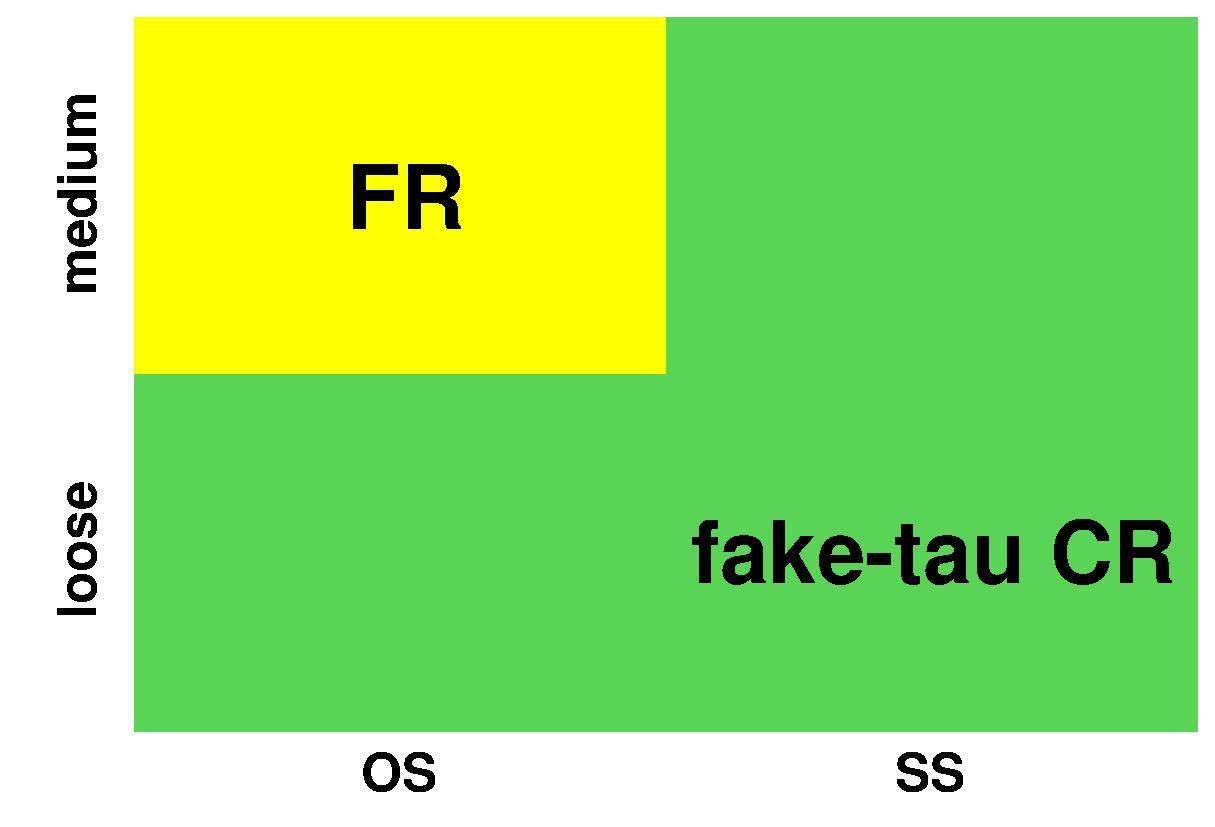
\includegraphics[width=0.45\textwidth]{figures/Htautau/fakes/fake-tau-control-region.eps}
%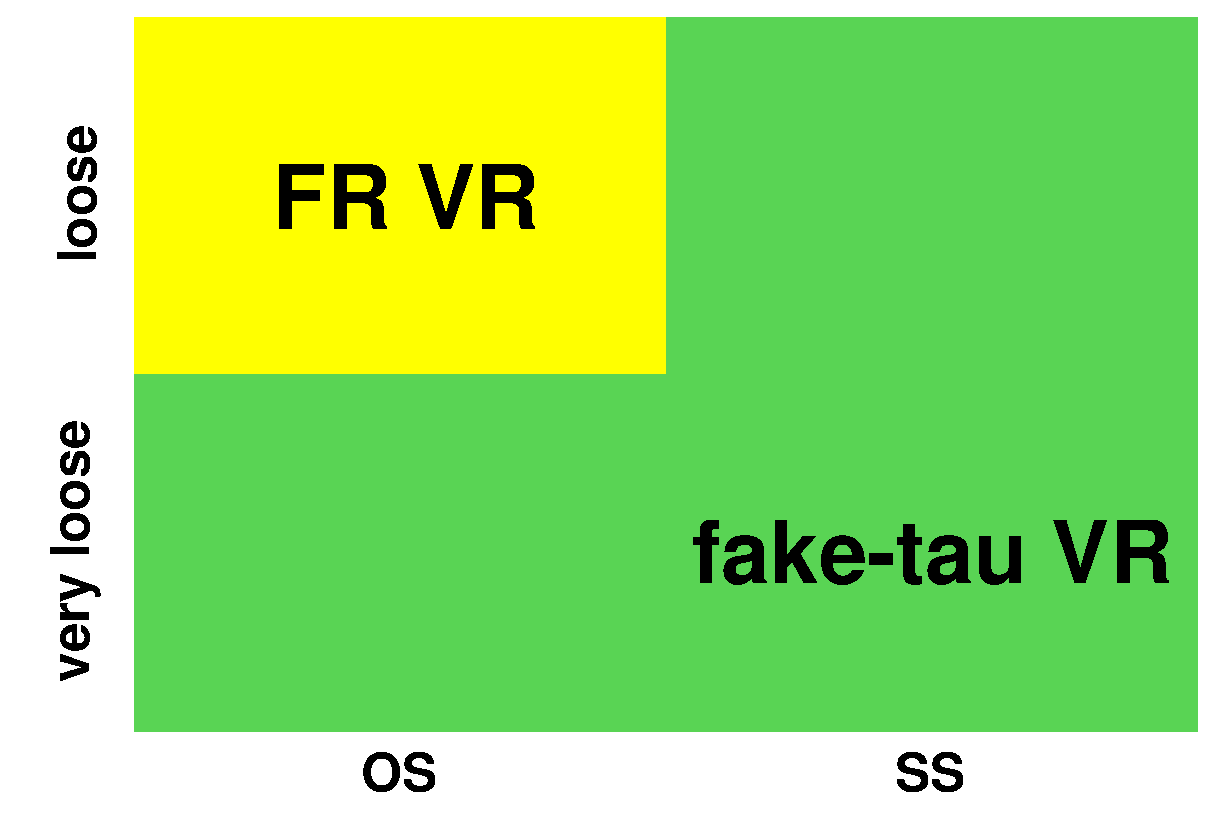
\includegraphics[width=0.45\textwidth]{figures/Htautau/fakes/VR.eps}
%
%\caption{ The composition of the FR, fake-tau CR, and corresponding VRs defined for the analysis. The ``Loose'', ``Medium'', ``very loose'' are leading (sub-leading) tau ID in $\lephad$ ($\hadhad$) channel. OS and SS represent the charge requirements of the tau candidates, OS for opposite sign, SS for same sign.}
%\label{fig:region-definition}
%\end{figure}
%
%In the fake-tau CR, the MC contaminations from $Z$+jets, diboson, top events ($\ttbar$, single top, $\ttbar+H/V$) with two real taus are subtracted, with only the QCD, $W$+jets and top fake events left. %The fake taus are those $\tauhad$ candidates which cannot be matched to any real taus in the MC truth.
%
%In the $\lephad$ channel, the top fake is the dominant fake background, and the fractions of top fake in FR and fake-tau CR are consistent with those in FR VR and fake-tau VR. The same is true for the fractions of $W$+jets in FR and fake-tau CR. Therefore, after the subtraction, the events in fake-tau CR are transferred to FR with a transfer factor, which is defined as
%
%\begin{equation}
%f_{\text{trans}} = \frac{N_{\text{data}}^{\text{FR}} - N_{\text{non-fake}}^{\text{FR}}}{N_{\text{fake}}^{\text{fake-tau-CR}}},
%\label{eq:transfer-factor}
%\end{equation}
%
%where $N_{\text{data}}^{\text{FR}}$ and $N_{\text{non-fake}}^{\text{FR}}$ are total event yields of data and non-fake MC background in FR, $N_{\text{fake}}^{\text{fake-tau-CR}}$ is the fake events from fake-tau CR, which is data-driven. Eq. \ref{eq:transfer-factor} gives a pre-fit normalization of the fake events to demonstrate the agreement of the data and total background prediction. After the fit, $f_{\text{trans}}$ will be modified by a new multiplicative factor (freely floating in the fit) replacting the final normalization of the fake. The fit untilizes the different distribution shapes of signal and background, as well as the background-enriched region in FR to determine the fake normalization.
%  
%In the $\hadhad$ channel, regarding that the QCD events have a considerable contribution to the fake-tau background and there is no guarentee that the fractions of top-fake-tau event in FR and fake-tau CR are the same. So a small amount of MC top-fake-tau events in fake-tau CR are added to the data-driven estimate to make them equal. The fractions of top-fake-tau events in both regions are simply computed by MC prediction. As a result, the fraction is also considered to have a systematic uncertainty (1-$\sigma$ deviation is around 30\%, which is measured in another top-enriched control region). So the transfer factor in the $\hadhad$ channel becomes:
%
%\begin{equation}
%f_{\text{trans}} = \frac{N_{\text{data}}^{\text{FR}} - N_{\text{non-fake}}^{\text{FR}}}{N_{\text{fake}}^{\text{fake-tau-CR}} + \epsilon N_{\text{topFake}}^{\text{fake-tau-CR}}},
%\label{eq:transfer-factor-hadhad}
%\end{equation}
%
%where $N_{\text{topFake}}^{\text{fake-tau CR}}$ is the top-fake-tau MC yield in fake-tau CR, and $\epsilon$ is a scaling factor that makes the top fake fractions equal in fake-tau CR and FR.
%
%To check if the shape of the BDT discriminant of the fake-tau events in fake-tau CR and in the FR agree with each other, independent FR and fake-tau CR validation regions (VR, as shown in Fig. \ref{fig:region-definition}) are defined. The VRs are basically the same as the nominal regions, except that
%
%\begin{itemize}
%\item The ``medium'' is downgraded to ``loose'', and ``loose'' downgraded to ``veryLoose'' for the subleading tau ID.
%\item In $\hadhad$, the ID of the leading $\tauhad$ is downgraded from ``medium'' to ``loose'' as well, in order to suppress the signal contamination.
%\end{itemize}
%
%The VRs are depleted of signals\footnote{The signal contamination is about $0.02\%$ and $0.15\%$ in the $\lephad$ 4-jet and $\hadhad$ 4-jet VRs, respectively, if assuming BR($t\to Hq$)=$1\%$.}, and the shape difference of the BDT discriminant of the fake-tau events between the FR VR and fake-tau VR (after subtracting on-fake MC backgrounds) are treated as one of the systematic uncertainty for the data-driven fake estimate.
%
%The different fractions of top fake, QCD and $W$+jets in fake-tau CR and FR can induce systematics in the fake estimation. In the $\lephad$ channel, relatively higher top fake fraction is seen in the FR than in the fake-tau CR. However, the top fake fractions in the FR and the FR VR are consistent with each other, and the same is true for the fractions in the fake-tau CR and the fake-tau VR. So the top fake fraction systematics is also covered by the VR samples comparisons.
